%!TEX root = ../../main.tex


\begin{figure}[p]
\centering
\vspace*{-10pt}
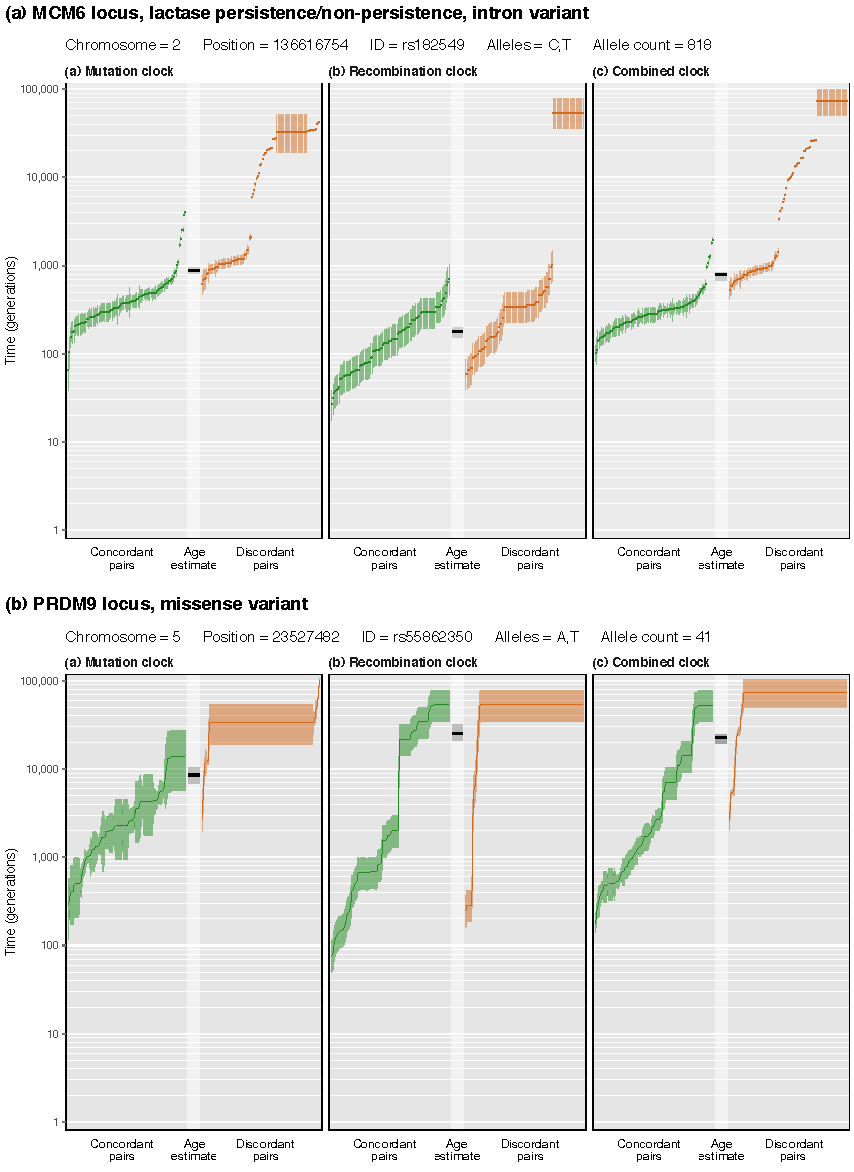
\includegraphics[width=\textwidth]{./img/ch5/1KG20_age_example}
\Caption{Example profiles of estimated allele age in 1000 Genomes, chromosome~20}%
{Allele age profiles are shown for \n{2} selected loci in \gls{1kg} data.
Each profile is composed of the \gls{tmrca} posterior distributions inferred for concordant pairs (\emph{left}) and discordant pairs (\emph{right}), which are sorted by their inferred \gls{tmrca}.
The estimated age obtained from the resulting composite posterior distribution is shown in the \emph{middle}.
Each \gls{tmrca} distribution is shown as the median, around which the \nth{1} and \nth{3} quartiles are drawn.
The mode of the composite posterior distribution is shown within a 95\% pseudo-confidence interval.
Time was scaled at $2\Ne$, where ${\Ne=\n{10000}}$.}%
{fig:1KG20_age_example}
\end{figure}
